\documentclass[ 12pt ]{article}
\usepackage{amsmath, amsthm, amssymb, csquotes, bbold, enumitem, extpfeil, graphicx, listings, mathrsfs, tikz-cd}
\usepackage[margin=0.5in]{geometry}

\usepackage{newunicodechar}

\newunicodechar{よ}{\text{\usefont{U}{min}{m}{n}\symbol{'210}}}

\DeclareFontFamily{U}{min}{}
\DeclareFontShape{U}{min}{m}{n}{<-> udmj30}{}

\graphicspath{ ./ }

\begin{document}

\noindent Landon Fox \\
\noindent Math 449, Category Theory and TQFTs \\
\noindent November 15, 2021

\begin{center}
\Large Homework 12
\end{center}

\begin{enumerate}

	% problem 1
	\item[\textbf{1.}] Prove that a vector space is dualizable if and only if it is finite dimensional.

		\begin{proof}
			For simplicity, we assume $\mathsf{Vect}_\mathbb{k}$ is strict monoidal by Mac Lane's Coherence Theorem. Let $V \in \mathsf{Vect}_\mathbb{k}$ be a finite dimensional vector space and $V^\ast \in \mathsf{Vect}_\mathbb{k}$ its dual. Then we obtain the nondegenerate evaluation pairing $\beta : V \otimes V^\ast \to \mathbb{k}$ and its copairing $\gamma : \mathbb{k} \to V^\ast \otimes V$. By definition of nondegeneracy, we obtain the following commutative diagrams
			\begin{center}
			\begin{tikzcd}
			V \arrow[rr, "\mathrm{id}_V \otimes \gamma"] \arrow[rrdd, "\mathrm{id}_V"'] &  & V \otimes V^\ast \otimes V \arrow[dd, "\beta \otimes \mathrm{id}_V"] &  & V^\ast \arrow[rr, "\gamma \otimes \mathrm{id}_{V^\ast}"] \arrow[rrdd, "\mathrm{id}_{V^\ast}"'] &  & V^\ast \otimes V \otimes V^\ast \arrow[dd, "\mathrm{id}_{V^\ast} \otimes \beta"] \\
			                                                                            &  &                                                                      &  &                                                                                                &  &                                                                                  \\
			                                                                            &  & V                                                                    &  &                                                                                                &  & V^\ast                                                                          
			\end{tikzcd}
			\end{center}
			as desired. \\

			Conversely, let $V \in \mathsf{Vect}_\mathbb{k}$ be dualizable; that is, we have a vector space $W \in \mathsf{Vect}_\mathbb{k}$, a pairing $\beta : V \otimes W \to \mathbb{k}$ and copairing $\gamma : \mathbb{k} \to W \otimes V$. By definition we have that $$\mathrm{id}_V = \beta \otimes \mathrm{id}_V \cdot \mathrm{id}_V \otimes \gamma.$$ If $\gamma(1) = \sum_{i=1}^n w_i \otimes v_i$ where $\{ w_i \}$ and $\{ v_i \}$ are, respectively, basis elements of $W$ and $V$, and $v \in V$ is an arbitrary vector, it follows that $$v = \mathrm{id}_V v = (\beta \otimes \mathrm{id}_V \cdot \mathrm{id}_V \otimes \gamma) v = \sum_{i=1}^n \beta(v \otimes w_i) v_i.$$ Since $\beta(v \otimes w_i) \in \mathbb{k}$ is a coefficient, we have that every $v \in V$ is in the span of $\{ v_i \}_{i \in [n]}$ and so $V$ is finite dimensional.
		\end{proof}


	% problem 2
	\item[\textbf{2.}] $ $
		\begin{enumerate}
			\item[\textbf{2.3.4.}] Show that if $A$ is a Frobenius algebra, then the handle operator $\mu \Delta : A \to A$ is a right $A$-module homomorphism.
			\item[\textbf{2.3.5.}] Show that the handle element is central.
		\end{enumerate}

		\begin{proof} $ $
			\begin{enumerate}
				\item[\textbf{2.3.4.}] Let $A$ be a Frobenius algebra. It suffices to show that the following diagram commutes;
				\begin{center}
				\begin{tikzcd}
				A \otimes A \arrow[rr, "\mu \Delta \otimes \mathrm{id}_A"] \arrow[dd, "\mu"'] &  & A \otimes A \arrow[dd, "\mu"] \\
				                                                                              &  &                               \\
				A \arrow[rr, "\mu \Delta"']                                                   &  & A                            
				\end{tikzcd}
				\end{center}
				we do so graphically. The linear map $\mu \cdot \mu \Delta \otimes \mathrm{id}_A$ can be expressed as
				\begin{center}
				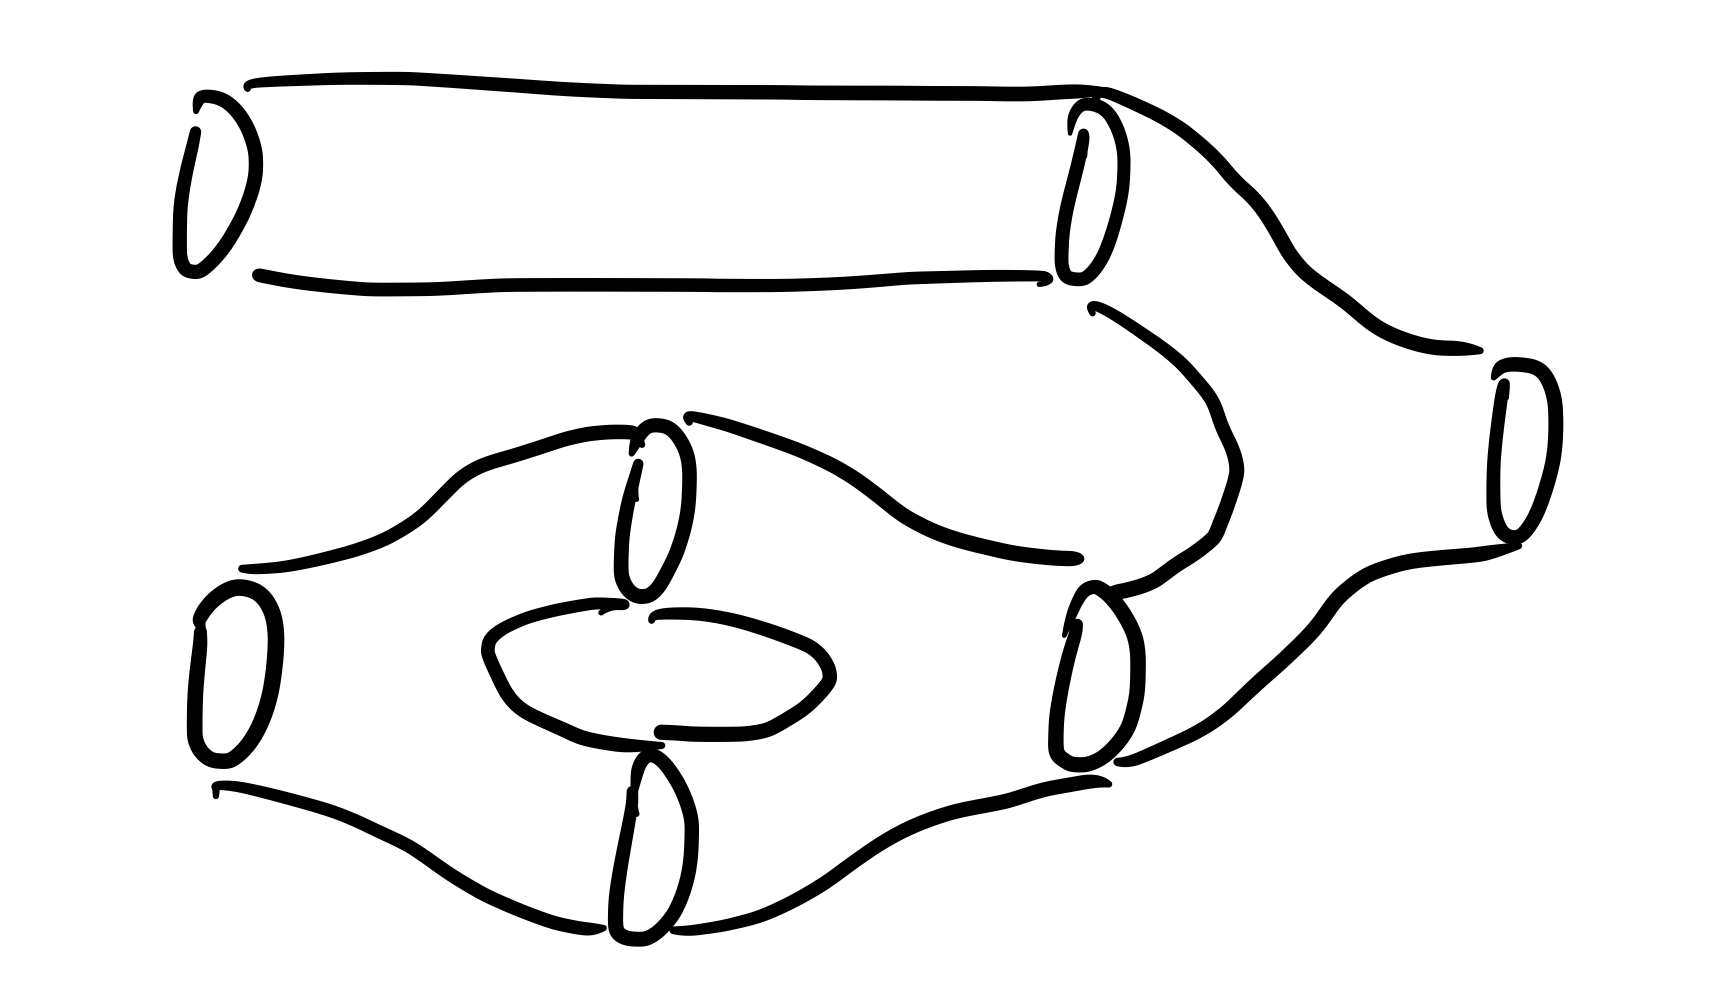
\includegraphics[scale=0.1]{Function}
				\end{center}
				Now observe that
				\begin{center}
				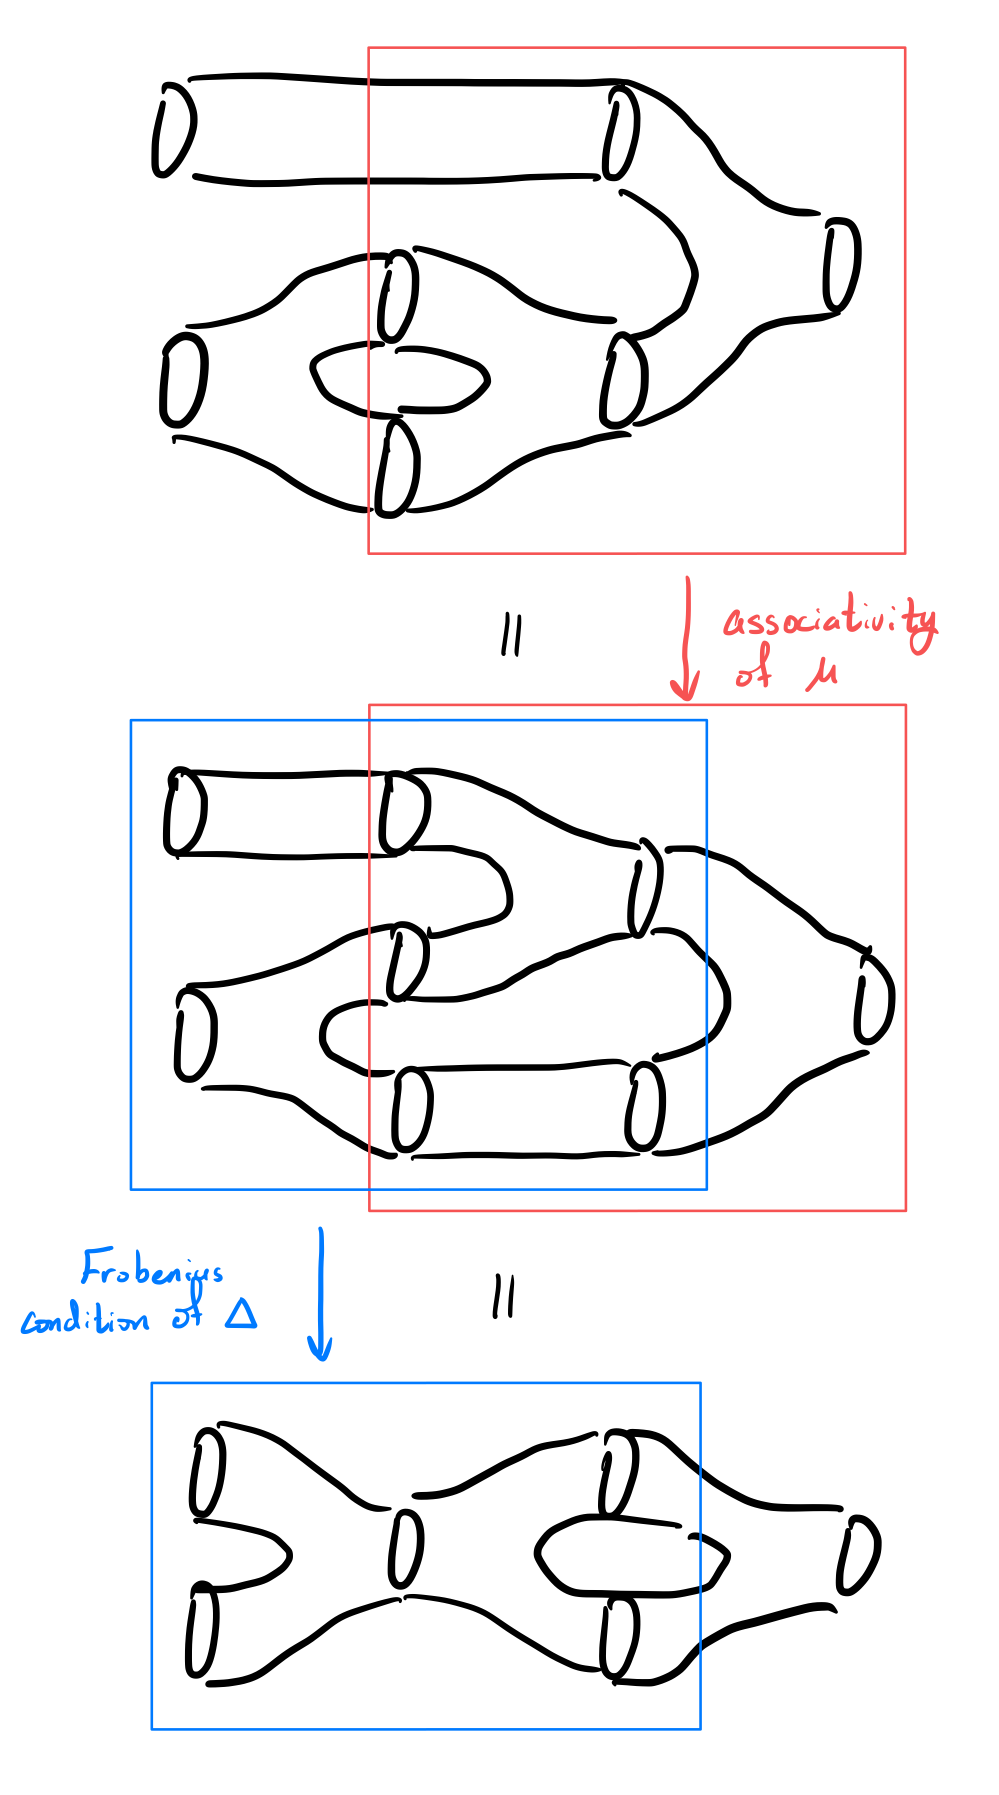
\includegraphics[scale=0.2]{Equality}
				\end{center}
				where the last surface represents $\mu \Delta \mu$. Thus, $\mu \Delta$ is a right $A$-module homomorphism.

				\item[\textbf{2.3.5.}] To show that the handle element is central, it suffices to show that
				\begin{center}
				\begin{tikzcd}
				A \otimes A \arrow[rr, "\mathrm{id}_A \otimes \mu \Delta"] \arrow[dd, "\mu"'] &  & A \otimes A \arrow[dd, "\mu"] \\
				                                                                              &  &                               \\
				A \arrow[rr, "\mu \Delta"']                                                   &  & A                            
				\end{tikzcd}
				\end{center}
				commutes; that is, we need
				\begin{center}
					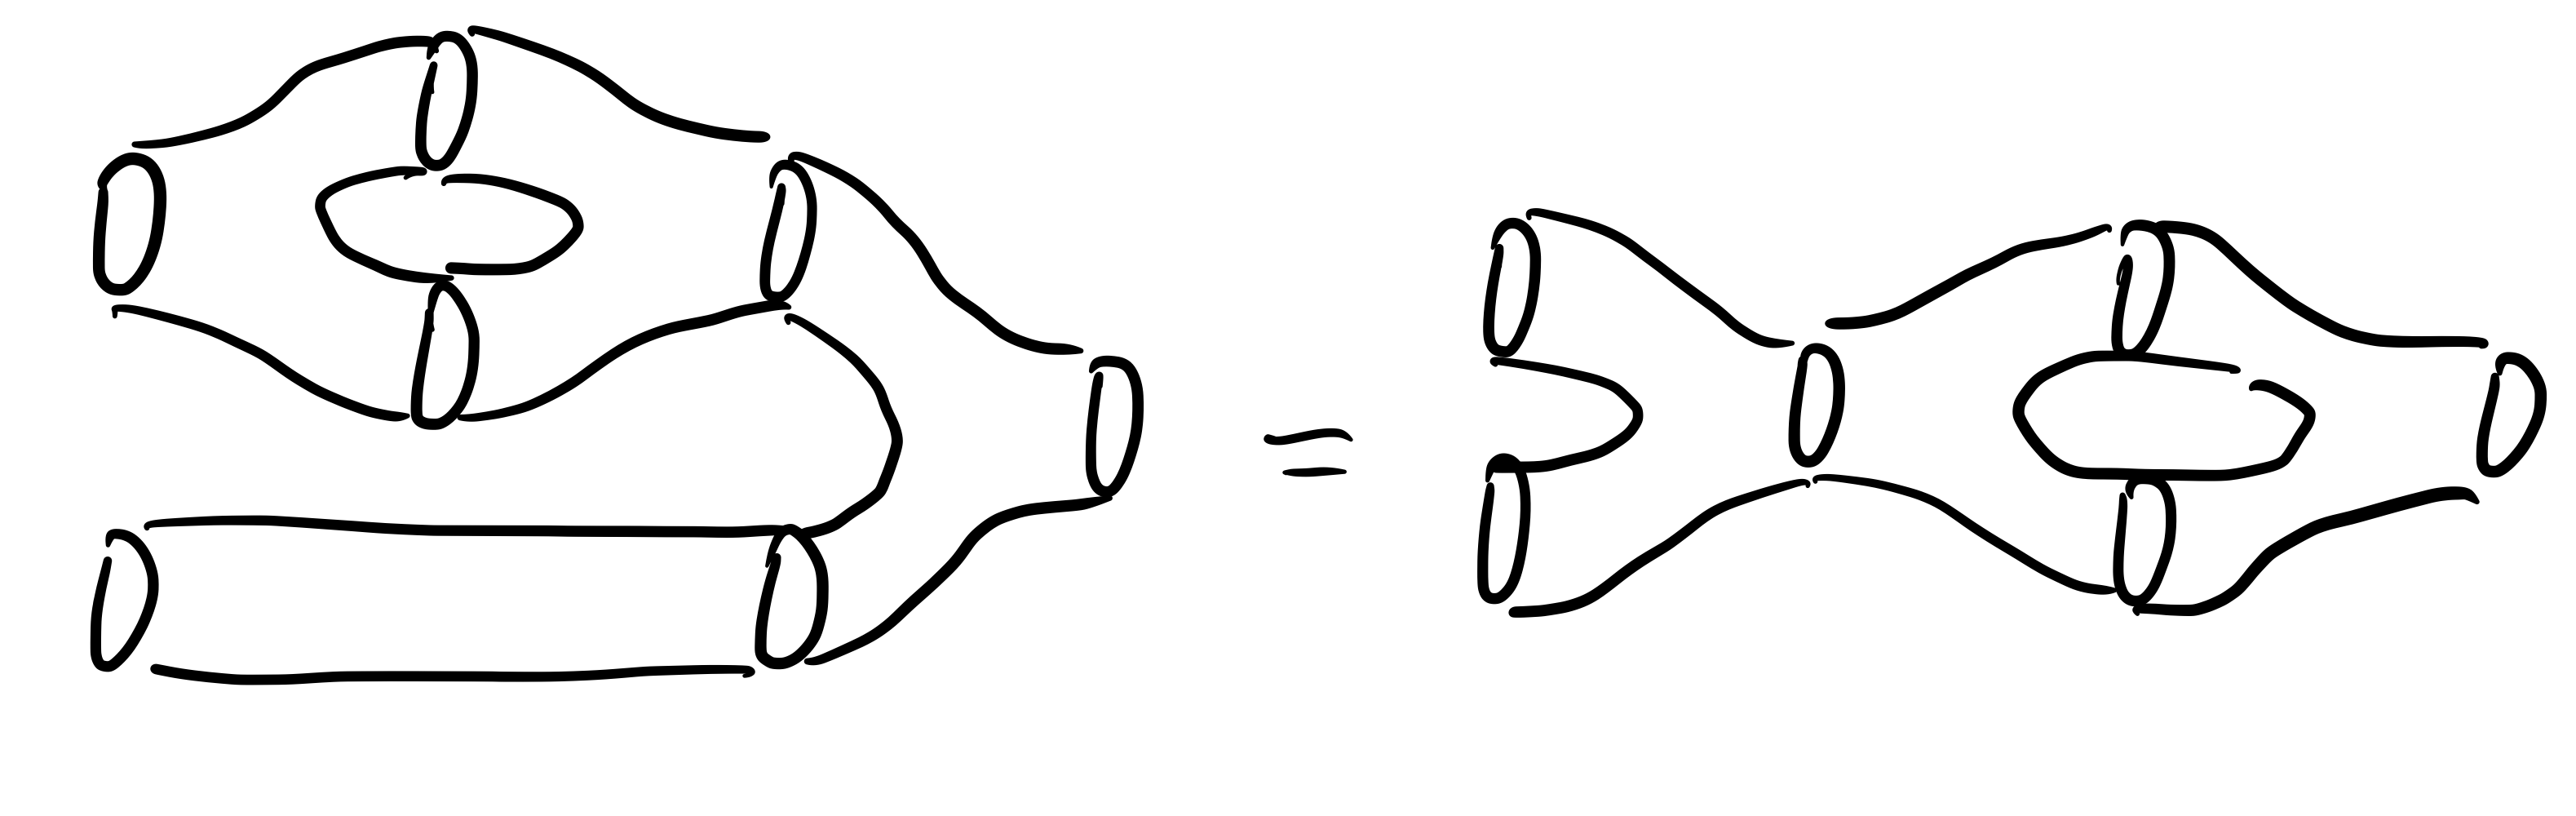
\includegraphics[scale=0.1]{goal}
				\end{center}
				Furthermore, observe that
				\begin{center}
					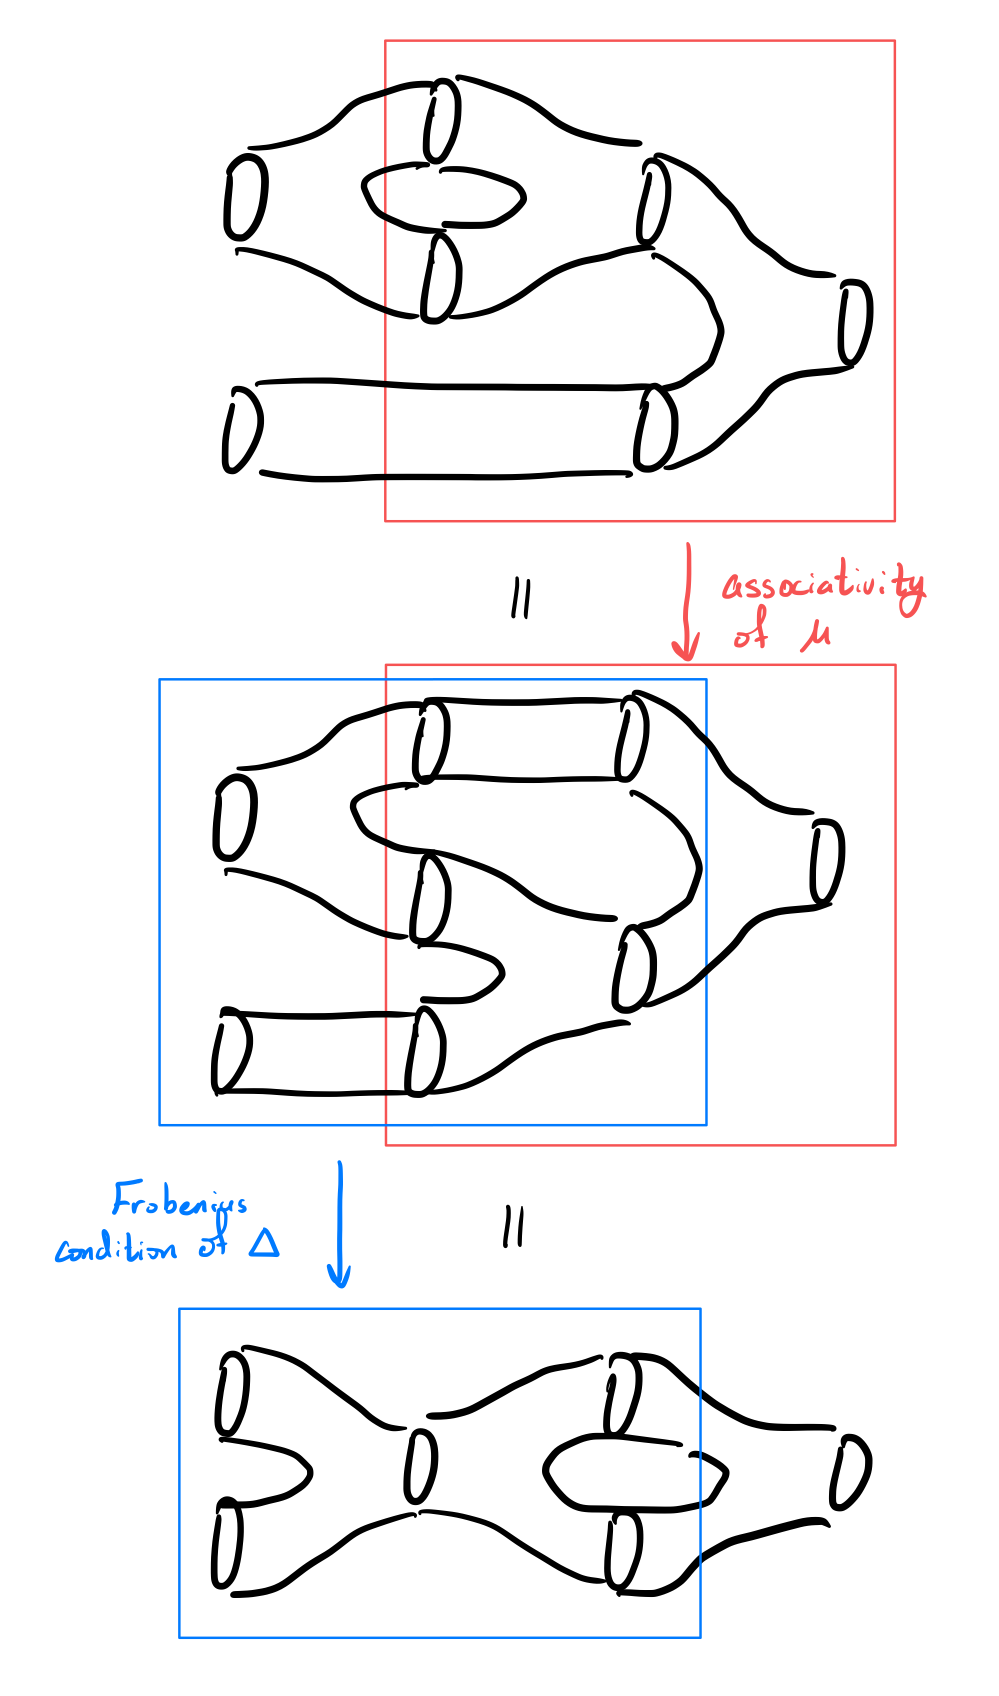
\includegraphics[scale=0.2]{equality2}
				\end{center}
				as desired.
			\end{enumerate}
		\end{proof}

\end{enumerate}

\end{document}
